\documentclass[12pt,a4paper]{article}
% Paquetes
\usepackage[utf8]{inputenc}\usepackage[T1]{fontenc}\usepackage[spanish]{babel}
\usepackage{amsmath,amssymb,mathtools,graphicx,geometry,float,pgfplots}\pgfplotsset{compat=1.18}
% Configuración de página
\geometry{a4paper,left=2.5cm,right=2.5cm,top=2.5cm,bottom=2.5cm}\setlength{\parindent}{1em}\setlength{\parskip}{0.3em}
% Datos de la entrega
\title{Entrega 5 Sistemas de Control}\author{Joaquín Basualdo\\Bautista Estrada\\Facundo Garaguso Fernandez}\date{Fecha de entrega: \today}
\begin{document}
% Portada
\maketitle\thispagestyle{plain}\newpage
% ===== EJERCICIO 2 =====
\section*{Ejercicio 2}
\begin{figure}[H] \centering 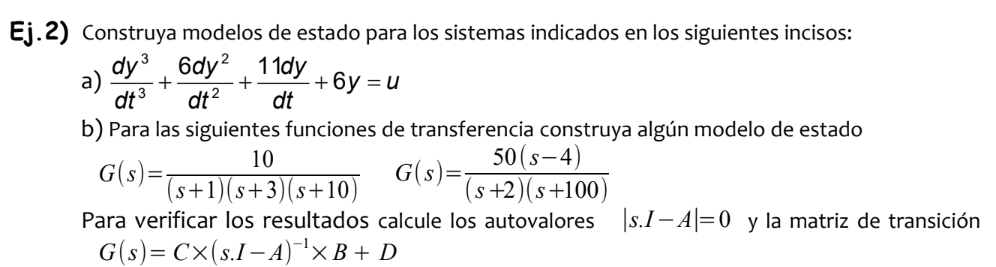
\includegraphics[width=\textwidth]{Imagenes/Ej2.png} \caption{Enunciado del Ejercicio 2.} \label{fig:enunciado_ej2} \end{figure}
Se construyen modelos de estado para los sistemas propuestos, utilizando la representación matricial:

\begin{equation}\dot{x}(t)=Ax(t)+Bu(t)\end{equation}

\begin{equation}y(t)=Cx(t)+Du(t)\end{equation}

Para verificar los modelos obtenidos se calculan los autovalores a partir de:

\begin{equation}\det(sI-A)=0\end{equation}

y se recupera la función de transferencia mediante:

\begin{equation}G(s)=C(sI-A)^{-1}B+D\end{equation}

Además, se obtiene la matriz de transición de estados en el dominio de Laplace:

\begin{equation}\Phi(s)=(sI-A)^{-1}\end{equation}

y su correspondiente expresión temporal:

\begin{equation}\Phi(t)=\mathcal{L}^{-1}\{\Phi(s)\}=e^{At}\end{equation}
% ===== INCISO A =====
\subsection*{a) Sistema definido por una ecuación diferencial}
Se parte de la siguiente ecuación diferencial:

\begin{equation}\frac{d^3y}{dt^3}+6\frac{d^2y}{dt^2}+11\frac{dy}{dt}+6y=u\end{equation}
\subsubsection*{Definición de las variables de estado}
Se definen las variables:

\begin{align}x_1&=y\\x_2&=\dot{x}_1=\dot{y}\\x_3&=\dot{x}_2=\ddot{y}\end{align}

Por lo tanto:

\begin{equation}\dot{x}_1=x_2\end{equation}

\begin{equation}\dot{x}_2=x_3\end{equation}

De la ecuación diferencial original:

\begin{equation}\dddot{y}=-6y-11\dot{y}-6\ddot{y}+u\end{equation}

Reemplazando las variables de estado:

\begin{equation}\dot{x}_3=-6x_1-11x_2-6x_3+u\end{equation}

En consecuencia, el sistema queda:

\begin{equation}\begin{cases}\dot{x}_1=x_2\\\dot{x}_2=x_3\\\dot{x}_3=-6x_1-11x_2-6x_3+u\end{cases}\end{equation}
\subsubsection*{Representación matricial}
Escribiendo las ecuaciones en forma matricial:

\begin{equation}\begin{bmatrix}\dot{x}_1\\\dot{x}_2\\\dot{x}_3\end{bmatrix}=\begin{bmatrix}0&1&0\\0&0&1\\-6&-11&-6\end{bmatrix} \begin{bmatrix}x_1\\x_2\\x_3\end{bmatrix}+\begin{bmatrix}0\\0\\1\end{bmatrix}u\end{equation}

Como la salida es $y=x_1$:

\begin{equation}y=\begin{bmatrix}1&0&0\end{bmatrix} \begin{bmatrix}x_1\\x_2\\x_3\end{bmatrix}+0u\end{equation}

Por lo tanto, las matrices del sistema son:

\begin{equation}\boxed{A=\begin{bmatrix}0&1&0\\0&0&1\\-6&-11&-6\end{bmatrix} \qquad B=\begin{bmatrix}0\\0\\1\end{bmatrix}}\end{equation}

\begin{equation}\boxed{C=\begin{bmatrix}1&0&0\end{bmatrix} \qquad D=0}\end{equation}

Se obtiene así una representación en forma canónica controlable.
\subsubsection*{Cálculo de autovalores}
Los autovalores se calculan mediante:

\begin{equation}\det(sI-A)=0\end{equation}

Primero:

\begin{equation}sI-A=\begin{bmatrix}s&-1&0\\0&s&-1\\6&11&s+6\end{bmatrix}\end{equation}

Calculando el determinante:

\begin{equation}\det(sI-A)=\begin{vmatrix}s&-1&0\\0&s&-1\\6&11&s+6\end{vmatrix}\end{equation}

Desarrollando por la primera fila:

\begin{align}\det(sI-A)&=s\left[s(s+6)+11\right]+6\\&=s^3+6s^2+11s+6\end{align}

Igualando a cero:

\begin{equation}s^3+6s^2+11s+6=0\end{equation}

Factorizando:

\begin{equation}(s+1)(s+2)(s+3)=0\end{equation}

Por lo tanto:

\begin{equation}\boxed{\lambda_1=-1,\qquad \lambda_2=-2,\qquad \lambda_3=-3}\end{equation}

Los tres autovalores son reales y negativos, por lo que el sistema es asintóticamente estable.
\subsubsection*{Matriz de transición de estados}
La matriz de transición en Laplace es:

\begin{equation}\Phi(s)=(sI-A)^{-1}\end{equation}

Reemplazando:

\begin{equation}\Phi(s)=\begin{bmatrix}s&-1&0\\0&s&-1\\6&11&s+6\end{bmatrix}^{-1}\end{equation}

Utilizando la expresión de la matriz inversa:

\begin{equation}Q^{-1}=\frac{\operatorname{adj}(Q)}{\det(Q)}\end{equation}

Se obtiene:

\begin{equation}\Phi(s)=\frac{1}{s^3+6s^2+11s+6} \begin{bmatrix}s^2+6s+11&s+6&1\\-6&s^2+6s&s\\-6s&-11s-6&s^2\end{bmatrix}\end{equation}

Como el denominador puede factorizarse:

\begin{equation}\boxed{\Phi(s)=\frac{1}{(s+1)(s+2)(s+3)} \begin{bmatrix}s^2+6s+11&s+6&1\\-6&s^2+6s&s\\-6s&-11s-6&s^2\end{bmatrix}}\end{equation}

Para obtener la matriz de transición temporal se aplica la transformada inversa de Laplace a cada elemento de la matriz.

Como los polos son simples, puede utilizarse una expansión en fracciones parciales matriciales:

\begin{equation}\Phi(s)=\frac{M_1}{s+1}+\frac{M_2}{s+2}+\frac{M_3}{s+3}\end{equation}

Calculando los residuos de cada término se obtiene:

\begin{equation}M_1=\frac{1}{2} \begin{bmatrix}6&5&1\\-6&-5&-1\\6&5&1\end{bmatrix}\end{equation}

\begin{equation}M_2=-\begin{bmatrix}3&4&1\\-6&-8&-2\\12&16&4\end{bmatrix}\end{equation}

\begin{equation}M_3=\frac{1}{2} \begin{bmatrix}2&3&1\\-6&-9&-3\\18&27&9\end{bmatrix}\end{equation}

Por lo tanto:

\begin{equation}\Phi(t)=M_1e^{-t}+M_2e^{-2t}+M_3e^{-3t}\end{equation}

Finalmente:

\begin{equation}\boxed{\begin{aligned}\Phi(t)={}&\frac{e^{-t}}{2} \begin{bmatrix}6&5&1\\-6&-5&-1\\6&5&1\end{bmatrix}\\[6pt]&-e^{-2t} \begin{bmatrix}3&4&1\\-6&-8&-2\\12&16&4\end{bmatrix}\\[6pt]&+\frac{e^{-3t}}{2} \begin{bmatrix}2&3&1\\-6&-9&-3\\18&27&9\end{bmatrix}\end{aligned}}\end{equation}

Se verifica que $\Phi(0)=I$.
\subsubsection*{Verificación de la función de transferencia}
Para comprobar el modelo:

\begin{equation}G(s)=C(sI-A)^{-1}B+D\end{equation}

Reemplazando las matrices:

\begin{equation}G(s)=\begin{bmatrix}1&0&0\end{bmatrix} \Phi(s) \begin{bmatrix}0\\0\\1\end{bmatrix}\end{equation}

Multiplicando la matriz de transición por $B$:

\begin{equation}\Phi(s)B=\frac{1}{s^3+6s^2+11s+6} \begin{bmatrix}1\\s\\s^2\end{bmatrix}\end{equation}

Luego:

\begin{equation}G(s)=\frac{1}{s^3+6s^2+11s+6} \begin{bmatrix}1&0&0\end{bmatrix} \begin{bmatrix}1\\s\\s^2\end{bmatrix}\end{equation}

En consecuencia:

\begin{equation}\boxed{G(s)=\frac{1}{s^3+6s^2+11s+6}}\end{equation}

Equivalentemente:

\begin{equation}\boxed{G(s)=\frac{1}{(s+1)(s+2)(s+3)}}\end{equation}

Se comprueba que corresponde a la transformada de Laplace de la ecuación diferencial original, considerando condiciones iniciales nulas.
% ===== INCISO B =====
\subsection*{b) Modelos de estado a partir de funciones de transferencia}
Para ambas funciones de transferencia se utiliza el método de desplazamiento de fase, obteniendo una representación en forma canónica controlable.
% ===== PRIMERA FUNCIÓN DE TRANSFERENCIA =====
\subsubsection*{Primera función de transferencia}
Se tiene:

\begin{equation}G(s)=\frac{10}{(s+1)(s+3)(s+10)}\end{equation}
\paragraph{Definición de las variables de estado.} Se introduce una variable intermedia $X_1(s)$, separando el denominador y el numerador:

\begin{equation}\frac{X_1(s)}{U(s)}=\frac{1}{(s+1)(s+3)(s+10)}\end{equation}

y:

\begin{equation}\frac{Y(s)}{X_1(s)}=10\end{equation}

Desarrollando el denominador:

\begin{align}&(s+1)(s+3)(s+10)\\&=(s^2+4s+3)(s+10)\\&=s^3+14s^2+43s+30\end{align}

Por lo tanto:

\begin{equation}X_1(s)(s^3+14s^2+43s+30)=U(s)\end{equation}

Aplicando transformada inversa de Laplace, con condiciones iniciales nulas para obtener la relación entrada-salida:

\begin{equation}\dddot{x}_1+14\ddot{x}_1+43\dot{x}_1+30x_1=u\end{equation}

Se definen:

\begin{align}x_2&=\dot{x}_1\\x_3&=\dot{x}_2=\ddot{x}_1\end{align}

En consecuencia:

\begin{equation}\dot{x}_1=x_2\end{equation}

\begin{equation}\dot{x}_2=x_3\end{equation}

Despejando la derivada de mayor orden:

\begin{equation}\dot{x}_3=-30x_1-43x_2-14x_3+u\end{equation}

La ecuación de salida se obtiene de:

\begin{equation}\frac{Y(s)}{X_1(s)}=10\end{equation}

Por lo tanto:

\begin{equation}y=10x_1\end{equation}
\paragraph{Representación matricial.} Escribiendo las ecuaciones:

\begin{equation}\begin{bmatrix}\dot{x}_1\\\dot{x}_2\\\dot{x}_3\end{bmatrix}=\begin{bmatrix}0&1&0\\0&0&1\\-30&-43&-14\end{bmatrix} \begin{bmatrix}x_1\\x_2\\x_3\end{bmatrix}+\begin{bmatrix}0\\0\\1\end{bmatrix}u\end{equation}

Y la salida:

\begin{equation}y=\begin{bmatrix}10&0&0\end{bmatrix} \begin{bmatrix}x_1\\x_2\\x_3\end{bmatrix}+0u\end{equation}

Por lo tanto:

\begin{equation}\boxed{A=\begin{bmatrix}0&1&0\\0&0&1\\-30&-43&-14\end{bmatrix} \qquad B=\begin{bmatrix}0\\0\\1\end{bmatrix}}\end{equation}

\begin{equation}\boxed{C=\begin{bmatrix}10&0&0\end{bmatrix} \qquad D=0}\end{equation}
\paragraph{Cálculo de autovalores.} Se plantea:

\begin{equation}\det(sI-A)=0\end{equation}

La matriz resulta:

\begin{equation}sI-A=\begin{bmatrix}s&-1&0\\0&s&-1\\30&43&s+14\end{bmatrix}\end{equation}

Calculando el determinante:

\begin{equation}\det(sI-A)=\begin{vmatrix}s&-1&0\\0&s&-1\\30&43&s+14\end{vmatrix}\end{equation}

Desarrollando:

\begin{align}\det(sI-A)&=s\left[s(s+14)+43\right]+30\\&=s^3+14s^2+43s+30\end{align}

Por lo tanto:

\begin{equation}s^3+14s^2+43s+30=0\end{equation}

Factorizando:

\begin{equation}(s+1)(s+3)(s+10)=0\end{equation}

Se obtienen los autovalores:

\begin{equation}\boxed{\lambda_1=-1,\qquad \lambda_2=-3,\qquad \lambda_3=-10}\end{equation}

Estos coinciden con los polos de la función de transferencia original. Como todos son negativos, el sistema es asintóticamente estable.
\paragraph{Matriz de transición de estados.} Se calcula:

\begin{equation}\Phi(s)=(sI-A)^{-1}\end{equation}

Reemplazando:

\begin{equation}\Phi(s)=\begin{bmatrix}s&-1&0\\0&s&-1\\30&43&s+14\end{bmatrix}^{-1}\end{equation}

Utilizando la matriz adjunta y el determinante:

\begin{equation}\Phi(s)=\frac{1}{s^3+14s^2+43s+30} \begin{bmatrix}s^2+14s+43&s+14&1\\-30&s^2+14s&s\\-30s&-43s-30&s^2\end{bmatrix}\end{equation}

Factorizando el denominador:

\begin{equation}\boxed{\Phi(s)=\frac{1}{(s+1)(s+3)(s+10)} \begin{bmatrix}s^2+14s+43&s+14&1\\-30&s^2+14s&s\\-30s&-43s-30&s^2\end{bmatrix}}\end{equation}

Para obtener la matriz de transición temporal, se aplica la transformada inversa de Laplace.

Como los polos son simples, se escribe:

\begin{equation}\Phi(s)=\frac{M_1}{s+1}+\frac{M_2}{s+3}+\frac{M_3}{s+10}\end{equation}

Los residuos matriciales son:

\begin{equation}M_1=\frac{1}{18} \begin{bmatrix}30&13&1\\-30&-13&-1\\30&13&1\end{bmatrix}\end{equation}

\begin{equation}M_2=-\frac{1}{14} \begin{bmatrix}10&11&1\\-30&-33&-3\\90&99&9\end{bmatrix}\end{equation}

\begin{equation}M_3=\frac{1}{63} \begin{bmatrix}3&4&1\\-30&-40&-10\\300&400&100\end{bmatrix}\end{equation}

Por lo tanto:

\begin{equation}\Phi(t)=M_1e^{-t}+M_2e^{-3t}+M_3e^{-10t}\end{equation}

Finalmente, la matriz de transición temporal es:

\begin{equation}\boxed{\begin{aligned}\Phi(t)={}&\frac{e^{-t}}{18} \begin{bmatrix}30&13&1\\-30&-13&-1\\30&13&1\end{bmatrix}\\[6pt]&-\frac{e^{-3t}}{14} \begin{bmatrix}10&11&1\\-30&-33&-3\\90&99&9\end{bmatrix}\\[6pt]&+\frac{e^{-10t}}{63} \begin{bmatrix}3&4&1\\-30&-40&-10\\300&400&100\end{bmatrix}\end{aligned}}\end{equation}

Se verifica que $\Phi(0)=I$.
\paragraph{Verificación de la función de transferencia.} A partir de las matrices obtenidas:

\begin{equation}G(s)=C(sI-A)^{-1}B+D\end{equation}

Como $D=0$:

\begin{equation}G(s)=\begin{bmatrix}10&0&0\end{bmatrix} \Phi(s) \begin{bmatrix}0\\0\\1\end{bmatrix}\end{equation}

Multiplicando:

\begin{equation}\Phi(s)B=\frac{1}{s^3+14s^2+43s+30} \begin{bmatrix}1\\s\\s^2\end{bmatrix}\end{equation}

Luego:

\begin{equation}G(s)=\frac{1}{s^3+14s^2+43s+30} \begin{bmatrix}10&0&0\end{bmatrix} \begin{bmatrix}1\\s\\s^2\end{bmatrix}\end{equation}

Se obtiene:

\begin{equation}G(s)=\frac{10}{s^3+14s^2+43s+30}\end{equation}

Finalmente:

\begin{equation}\boxed{G(s)=\frac{10}{(s+1)(s+3)(s+10)}}\end{equation}

La expresión coincide exactamente con la función de transferencia propuesta, verificando el modelo de estado obtenido.
% ===== SEGUNDA FUNCIÓN DE TRANSFERENCIA =====
\subsubsection*{Segunda función de transferencia}
Se tiene:

\begin{equation}G(s)=\frac{50(s-4)}{(s+2)(s+100)}\end{equation}
\paragraph{Definición de las variables de estado.} Se introduce una variable intermedia $X_1(s)$, separando la función de transferencia:

\begin{equation}\frac{X_1(s)}{U(s)}=\frac{1}{(s+2)(s+100)}\end{equation}

y:

\begin{equation}\frac{Y(s)}{X_1(s)}=50(s-4)\end{equation}

Desarrollando el denominador:

\begin{equation}(s+2)(s+100)=s^2+102s+200\end{equation}

De esta manera:

\begin{equation}X_1(s)(s^2+102s+200)=U(s)\end{equation}

Aplicando transformada inversa de Laplace, considerando condiciones iniciales nulas:

\begin{equation}\ddot{x}_1+102\dot{x}_1+200x_1=u\end{equation}

Se define:

\begin{equation}x_2=\dot{x}_1\end{equation}

Por lo tanto:

\begin{equation}\dot{x}_1=x_2\end{equation}

Despejando la segunda derivada:

\begin{equation}\ddot{x}_1=-200x_1-102\dot{x}_1+u\end{equation}

Reemplazando:

\begin{equation}\dot{x}_2=-200x_1-102x_2+u\end{equation}

Para determinar la salida, se utiliza:

\begin{equation}\frac{Y(s)}{X_1(s)}=50(s-4)\end{equation}

Por lo tanto:

\begin{equation}Y(s)=(50s-200)X_1(s)\end{equation}

En el dominio temporal:

\begin{equation}y=50\dot{x}_1-200x_1\end{equation}

Como $\dot{x}_1=x_2$:

\begin{equation}\boxed{y=-200x_1+50x_2}\end{equation}

Así, el sistema de ecuaciones queda:

\begin{equation}\begin{cases}\dot{x}_1=x_2\\\dot{x}_2=-200x_1-102x_2+u\\y=-200x_1+50x_2\end{cases}\end{equation}
\paragraph{Representación matricial.} Escribiendo las ecuaciones:

\begin{equation}\begin{bmatrix}\dot{x}_1\\\dot{x}_2\end{bmatrix}=\begin{bmatrix}0&1\\-200&-102\end{bmatrix} \begin{bmatrix}x_1\\x_2\end{bmatrix}+\begin{bmatrix}0\\1\end{bmatrix}u\end{equation}

La salida es:

\begin{equation}y=\begin{bmatrix}-200&50\end{bmatrix} \begin{bmatrix}x_1\\x_2\end{bmatrix}+0u\end{equation}

Por lo tanto:

\begin{equation}\boxed{A=\begin{bmatrix}0&1\\-200&-102\end{bmatrix} \qquad B=\begin{bmatrix}0\\1\end{bmatrix}}\end{equation}

\begin{equation}\boxed{C=\begin{bmatrix}-200&50\end{bmatrix} \qquad D=0}\end{equation}

Esta representación también corresponde a la forma canónica controlable.
\paragraph{Cálculo de autovalores.} Se plantea:

\begin{equation}\det(sI-A)=0\end{equation}

Primero:

\begin{equation}sI-A=\begin{bmatrix}s&-1\\200&s+102\end{bmatrix}\end{equation}

El determinante es:

\begin{equation}\det(sI-A)=\begin{vmatrix}s&-1\\200&s+102\end{vmatrix}\end{equation}

Desarrollando:

\begin{align}\det(sI-A)&=s(s+102)+200\\&=s^2+102s+200\end{align}

Igualando a cero:

\begin{equation}s^2+102s+200=0\end{equation}

Factorizando:

\begin{equation}(s+2)(s+100)=0\end{equation}

Se obtienen los autovalores:

\begin{equation}\boxed{\lambda_1=-2,\qquad \lambda_2=-100}\end{equation}

Ambos autovalores son reales y negativos, por lo que el sistema es asintóticamente estable.
\paragraph{Matriz de transición de estados.} Se calcula:

\begin{equation}\Phi(s)=(sI-A)^{-1}\end{equation}

Reemplazando:

\begin{equation}\Phi(s)=\begin{bmatrix}s&-1\\200&s+102\end{bmatrix}^{-1}\end{equation}

Utilizando la fórmula de la inversa para una matriz de $2\times2$:

\begin{equation}\begin{bmatrix}a&b\\c&d\end{bmatrix}^{-1}=\frac{1}{ad-bc} \begin{bmatrix}d&-b\\-c&a\end{bmatrix}\end{equation}

Se obtiene:

\begin{equation}\Phi(s)=\frac{1}{s(s+102)+200} \begin{bmatrix}s+102&1\\-200&s\end{bmatrix}\end{equation}

Factorizando:

\begin{equation}\boxed{\Phi(s)=\frac{1}{(s+2)(s+100)} \begin{bmatrix}s+102&1\\-200&s\end{bmatrix}}\end{equation}

Para obtener la matriz de transición temporal se aplica la transformada inversa de Laplace a cada elemento.

Se comienza desarrollando en fracciones parciales.

Para el elemento $(1,1)$:

\begin{equation}\frac{s+102}{(s+2)(s+100)}=\frac{50/49}{s+2}-\frac{1/49}{s+100}\end{equation}

Para el elemento $(1,2)$:

\begin{equation}\frac{1}{(s+2)(s+100)}=\frac{1/98}{s+2}-\frac{1/98}{s+100}\end{equation}

Para el elemento $(2,1)$:

\begin{equation}\frac{-200}{(s+2)(s+100)}=-\frac{100/49}{s+2}+\frac{100/49}{s+100}\end{equation}

Finalmente, para el elemento $(2,2)$:

\begin{equation}\frac{s}{(s+2)(s+100)}=-\frac{1/49}{s+2}+\frac{50/49}{s+100}\end{equation}

Aplicando transformada inversa de Laplace:

\begin{equation}\boxed{\Phi(t)=\frac{1}{98} \begin{bmatrix}100e^{-2t}-2e^{-100t}&e^{-2t}-e^{-100t}\\[6pt]-200e^{-2t}+200e^{-100t}&-2e^{-2t}+100e^{-100t}\end{bmatrix}}\end{equation}

Se verifica que para $t=0$:

\begin{equation}\Phi(0)=\frac{1}{98} \begin{bmatrix}98&0\\0&98\end{bmatrix}\end{equation}

Por lo tanto:

\begin{equation}\boxed{\Phi(0)=I}\end{equation}
\paragraph{Verificación de la función de transferencia.} Se utiliza:

\begin{equation}G(s)=C(sI-A)^{-1}B+D\end{equation}

Como $D=0$:

\begin{equation}G(s)=\begin{bmatrix}-200&50\end{bmatrix} \Phi(s) \begin{bmatrix}0\\1\end{bmatrix}\end{equation}

Reemplazando la matriz de transición:

\begin{equation}G(s)=\frac{1}{(s+2)(s+100)} \begin{bmatrix}-200&50\end{bmatrix} \begin{bmatrix}s+102&1\\-200&s\end{bmatrix} \begin{bmatrix}0\\1\end{bmatrix}\end{equation}

Multiplicando primero la matriz por $B$:

\begin{equation}\begin{bmatrix}s+102&1\\-200&s\end{bmatrix} \begin{bmatrix}0\\1\end{bmatrix}=\begin{bmatrix}1\\s\end{bmatrix}\end{equation}

Por lo tanto:

\begin{equation}G(s)=\frac{1}{(s+2)(s+100)} \begin{bmatrix}-200&50\end{bmatrix} \begin{bmatrix}1\\s\end{bmatrix}\end{equation}

Realizando el producto:

\begin{equation}G(s)=\frac{-200+50s}{(s+2)(s+100)}\end{equation}

Sacando factor común:

\begin{equation}\boxed{G(s)=\frac{50(s-4)}{(s+2)(s+100)}}\end{equation}

La función de transferencia obtenida coincide exactamente con la original, verificando que las matrices $A$, $B$, $C$ y $D$ representan correctamente al sistema.
% ===== EJERCICIO 3 =====
\section*{Ejercicio 3}
\begin{figure}[H] \centering 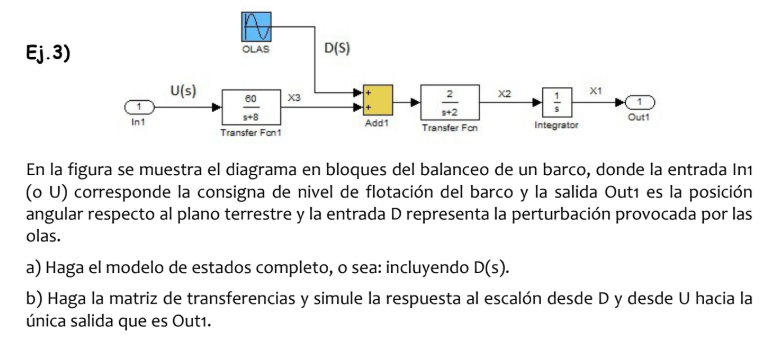
\includegraphics[width=\textwidth]{Imagenes/Ej3.png} \caption{Enunciado y diagrama de bloques del Ejercicio 3.} \label{fig:enunciado_ej3} \end{figure}
Se estudia el sistema de balanceo de un barco representado mediante un diagrama de bloques.

El sistema cuenta con dos entradas: la señal de control $u(t)$, correspondiente a la consigna del sistema, y la perturbación $d(t)$, que representa el efecto de las olas sobre el barco.

La salida $y(t)$ corresponde a la posición angular del barco respecto del plano terrestre.

Se pide:

\begin{enumerate}
\item Construir el modelo de estado completo, incluyendo la perturbación $d(t)$.
\item Obtener la matriz de transferencias y simular la respuesta al escalón desde cada una de las entradas hacia la salida.
\end{enumerate}
% ===== INCISO A =====
\subsection*{a) Modelo de estado completo}
Para construir el modelo se utiliza el método de desplazamiento de fase, tomando como variables de estado las salidas de los tres bloques dinámicos del sistema.

De acuerdo con el diagrama de bloques, las transferencias que conforman el sistema son:

\begin{equation}G_1(s)=\frac{60}{s+8}\end{equation}

\begin{equation}G_2(s)=\frac{2}{s+2}\end{equation}

\begin{equation}G_3(s)=\frac{1}{s}\end{equation}

Se definen las siguientes variables de estado:

\begin{itemize}
\item $x_3$: salida del primer bloque, cuya transferencia es $60/(s+8)$.
\item $x_2$: salida del segundo bloque, cuya transferencia es $2/(s+2)$.
\item $x_1$: salida del integrador, que coincide con la salida del sistema.
\end{itemize}
\subsubsection*{Obtención de las ecuaciones de estado}
\paragraph{Primera etapa: bloque de transferencia $\boldsymbol{60/(s+8)}$.} Del diagrama se observa que:

\begin{equation}X_3(s)=U(s)\frac{60}{s+8}\end{equation}

Reordenando:

\begin{equation}(s+8)X_3(s)=60U(s)\end{equation}

Desarrollando:

\begin{equation}sX_3(s)+8X_3(s)=60U(s)\end{equation}

Aplicando transformada inversa de Laplace, considerando condiciones iniciales nulas:

\begin{equation}\dot{x}_3+8x_3=60u\end{equation}

Despejando:

\begin{equation}\boxed{\dot{x}_3=-8x_3+60u}\end{equation}
\paragraph{Segunda etapa: bloque de transferencia $\boldsymbol{2/(s+2)}$.} En este bloque se suman la señal $x_3$ proveniente del primer bloque y la perturbación $d(t)$ producida por las olas.

Por lo tanto:

\begin{equation}X_2(s)=\left[X_3(s)+D_{\mathrm{olas}}(s)\right] \frac{2}{s+2}\end{equation}

Multiplicando:

\begin{equation}(s+2)X_2(s)=2X_3(s)+2D_{\mathrm{olas}}(s)\end{equation}

Desarrollando:

\begin{equation}sX_2(s)+2X_2(s)=2X_3(s)+2D_{\mathrm{olas}}(s)\end{equation}

Aplicando transformada inversa de Laplace:

\begin{equation}\dot{x}_2+2x_2=2x_3+2d\end{equation}

Finalmente:

\begin{equation}\boxed{\dot{x}_2=-2x_2+2x_3+2d}\end{equation}
\paragraph{Tercera etapa: bloque integrador $\boldsymbol{1/s}$.} Para el último bloque:

\begin{equation}X_1(s)=\frac{X_2(s)}{s}\end{equation}

Reordenando:

\begin{equation}sX_1(s)=X_2(s)\end{equation}

Aplicando transformada inversa de Laplace:

\begin{equation}\boxed{\dot{x}_1=x_2}\end{equation}

Como la salida del sistema coincide con la salida del integrador:

\begin{equation}\boxed{y=x_1}\end{equation}
\subsubsection*{Sistema de ecuaciones obtenido}
Reuniendo las ecuaciones anteriores:

\begin{equation}\boxed{\begin{cases}\dot{x}_1=x_2\\\dot{x}_2=-2x_2+2x_3+2d\\\dot{x}_3=-8x_3+60u\\y=x_1\end{cases}}\end{equation}

Se observa que la entrada de control $u$ actúa sobre la dinámica de $x_3$, mientras que la perturbación $d$ ingresa directamente en la dinámica de $x_2$.
\subsubsection*{Representación matricial}
El modelo completo se expresa como:

\begin{equation}\dot{x}=Ax+Bw\end{equation}

donde el vector de entradas es:

\begin{equation}w(t)=\begin{bmatrix}u(t)\\d(t)\end{bmatrix}\end{equation}

Escribiendo las ecuaciones en forma matricial:

\begin{equation}\begin{bmatrix}\dot{x}_1\\\dot{x}_2\\\dot{x}_3\end{bmatrix}=\begin{bmatrix}0&1&0\\0&-2&2\\0&0&-8\end{bmatrix} \begin{bmatrix}x_1\\x_2\\x_3\end{bmatrix}+\begin{bmatrix}0&0\\0&2\\60&0\end{bmatrix} \begin{bmatrix}u\\d\end{bmatrix}\end{equation}

La salida queda definida por:

\begin{equation}y=\begin{bmatrix}1&0&0\end{bmatrix} \begin{bmatrix}x_1\\x_2\\x_3\end{bmatrix}+\begin{bmatrix}0&0\end{bmatrix} \begin{bmatrix}u\\d\end{bmatrix}\end{equation}

Por lo tanto, las matrices del sistema son:

\begin{equation}\boxed{A=\begin{bmatrix}0&1&0\\0&-2&2\\0&0&-8\end{bmatrix}}\end{equation}

\begin{equation}\boxed{B=\begin{bmatrix}0&0\\0&2\\60&0\end{bmatrix}}\end{equation}

\begin{equation}\boxed{C=\begin{bmatrix}1&0&0\end{bmatrix} \qquad D=\begin{bmatrix}0&0\end{bmatrix}}\end{equation}

La matriz $B$ posee dos columnas debido a que el sistema tiene dos entradas.

La primera columna representa la acción de la entrada de control $u$, mientras que la segunda corresponde a la perturbación $d$.

La matriz $C$ selecciona la primera variable de estado, dado que la única salida del sistema es $y=x_1$.
% ===== INCISO B =====
\subsection*{b) Matriz de transferencias y respuestas al escalón}
Se busca obtener la relación entre las dos entradas del sistema y la única salida.

La representación general en el dominio de Laplace es:

\begin{equation}Y(s)=G_u(s)U(s)+G_d(s)D_{\mathrm{olas}}(s)\end{equation}

Por lo tanto, la matriz de transferencias será una matriz de dimensión $1\times2$:

\begin{equation}G(s)=\begin{bmatrix}G_u(s)&G_d(s)\end{bmatrix}\end{equation}
\subsubsection*{Obtención de las transferencias a partir del diagrama de bloques}
\paragraph{Transferencia desde la entrada de control.} Para calcular la relación entre la entrada $u$ y la salida $y$, se considera nula la perturbación:

\begin{equation}d(t)=0\end{equation}

Del diagrama de bloques, los tres bloques dinámicos quedan conectados en cascada.

Por lo tanto:

\begin{equation}G_u(s)=\frac{60}{s+8} \frac{2}{s+2} \frac{1}{s}\end{equation}

Multiplicando:

\begin{equation}\boxed{G_u(s)=\frac{120}{s(s+2)(s+8)}}\end{equation}

Desarrollando el denominador:

\begin{equation}s(s+2)(s+8)=s^3+10s^2+16s\end{equation}

De esta manera:

\begin{equation}G_u(s)=\frac{120}{s^3+10s^2+16s}\end{equation}
\paragraph{Transferencia desde la perturbación.} Para obtener la transferencia entre la perturbación $d$ y la salida $y$, se considera nula la entrada de control:

\begin{equation}u(t)=0\end{equation}

La perturbación ingresa directamente antes del segundo bloque, por lo que solamente atraviesa las transferencias $2/(s+2)$ y $1/s$.

Entonces:

\begin{equation}G_d(s)=\frac{2}{s+2}\frac{1}{s}\end{equation}

Finalmente:

\begin{equation}\boxed{G_d(s)=\frac{2}{s(s+2)}}\end{equation}
\subsubsection*{Matriz de transferencias}
Reuniendo ambas expresiones:

\begin{equation}\boxed{G(s)=\begin{bmatrix}\dfrac{120}{s(s+2)(s+8)}&\dfrac{2}{s(s+2)}\end{bmatrix}}\end{equation}

Esta matriz permite determinar la salida del sistema para cualquier combinación de ambas entradas, considerando condiciones iniciales nulas.
\subsubsection*{Verificación mediante el modelo de estados}
Se verifica la matriz de transferencias utilizando la expresión:

\begin{equation}G(s)=C(sI-A)^{-1}B+D\end{equation}

En primer lugar se calcula:

\begin{equation}sI-A=\begin{bmatrix}s&-1&0\\0&s+2&-2\\0&0&s+8\end{bmatrix}\end{equation}

Como la matriz es triangular superior, su determinante es el producto de los elementos de la diagonal:

\begin{equation}\det(sI-A)=s(s+2)(s+8)\end{equation}

La inversa resulta:

\begin{equation}(sI-A)^{-1}=\begin{bmatrix}\dfrac{1}{s}&\dfrac{1}{s(s+2)}&\dfrac{2}{s(s+2)(s+8)}\\[8pt]0&\dfrac{1}{s+2}&\dfrac{2}{(s+2)(s+8)}\\[8pt]0&0&\dfrac{1}{s+8}\end{bmatrix}\end{equation}

Reemplazando en la expresión de la matriz de transferencias:

\begin{equation}G(s)=C(sI-A)^{-1}B+D\end{equation}

Como $D=0$:

\begin{equation}G(s)=\begin{bmatrix}1&0&0\end{bmatrix} (sI-A)^{-1} \begin{bmatrix}0&0\\0&2\\60&0\end{bmatrix}\end{equation}

Multiplicando primero $C$ por la inversa:

\begin{equation}C(sI-A)^{-1}=\begin{bmatrix}\dfrac{1}{s}&\dfrac{1}{s(s+2)}&\dfrac{2}{s(s+2)(s+8)}\end{bmatrix}\end{equation}

Luego:

\begin{equation}G(s)=\begin{bmatrix}\dfrac{1}{s}&\dfrac{1}{s(s+2)}&\dfrac{2}{s(s+2)(s+8)}\end{bmatrix} \begin{bmatrix}0&0\\0&2\\60&0\end{bmatrix}\end{equation}

Realizando el producto matricial:

\begin{equation}\boxed{G(s)=\begin{bmatrix}\dfrac{120}{s(s+2)(s+8)}&\dfrac{2}{s(s+2)}\end{bmatrix}}\end{equation}

El resultado coincide con las transferencias obtenidas directamente del diagrama de bloques.

Por lo tanto, se verifica el modelo de estados construido en el inciso a).
% ===== AUTOVALORES =====
\subsubsection*{Análisis de los autovalores}
Para analizar la dinámica del sistema, se calculan los autovalores de la matriz $A$.

La ecuación característica es:

\begin{equation}\det(sI-A)=0\end{equation}

Como se obtuvo anteriormente:

\begin{equation}s(s+2)(s+8)=0\end{equation}

Por lo tanto:

\begin{equation}\boxed{\lambda_1=0,\qquad \lambda_2=-2,\qquad \lambda_3=-8}\end{equation}

El sistema presenta dos polos reales negativos y un polo ubicado en el origen.

El polo en el origen corresponde al integrador presente en el diagrama de bloques.

Por este motivo, el sistema no es asintóticamente estable y no alcanza un valor estacionario finito frente a un escalón unitario.
% ===== RESPUESTA AL ESCALÓN DESDE U =====
\subsubsection*{Respuesta al escalón desde la entrada de control}
Se considera un escalón unitario aplicado a la entrada de control:

\begin{equation}u(t)=1,\qquad t\geq0\end{equation}

Y se anula la perturbación:

\begin{equation}d(t)=0\end{equation}

La transformada de Laplace de la entrada es:

\begin{equation}U(s)=\frac{1}{s}\end{equation}

La salida está dada por:

\begin{equation}Y_u(s)=G_u(s)U(s)\end{equation}

Reemplazando:

\begin{equation}Y_u(s)=\frac{120}{s(s+2)(s+8)} \frac{1}{s}\end{equation}

Por lo tanto:

\begin{equation}\boxed{Y_u(s)=\frac{120}{s^2(s+2)(s+8)}}\end{equation}
\paragraph{Descomposición en fracciones parciales.} Se propone:

\begin{equation}\frac{120}{s^2(s+2)(s+8)}=\frac{A_1}{s}+\frac{A_2}{s^2}+\frac{A_3}{s+2}+\frac{A_4}{s+8}\end{equation}

Calculando los coeficientes:

\begin{equation}A_2=\left. \frac{120}{(s+2)(s+8)} \right|_{s=0}=\frac{15}{2}\end{equation}

Para el coeficiente del término $1/s$:

\begin{equation}A_1=\left. \frac{d}{ds} \left( \frac{120}{(s+2)(s+8)} \right) \right|_{s=0}\end{equation}

Resultando:

\begin{equation}A_1=-\frac{75}{16}\end{equation}

Para los otros coeficientes:

\begin{equation}A_3=\left. \frac{120}{s^2(s+8)} \right|_{s=-2}=5\end{equation}

\begin{equation}A_4=\left. \frac{120}{s^2(s+2)} \right|_{s=-8}=-\frac{5}{16}\end{equation}

Por lo tanto:

\begin{equation}Y_u(s)=-\frac{75}{16s}+\frac{15}{2s^2}+\frac{5}{s+2}-\frac{5}{16(s+8)}\end{equation}

Aplicando transformada inversa de Laplace:

\begin{equation}\boxed{y_u(t)=\frac{15}{2}t-\frac{75}{16}+5e^{-2t}-\frac{5}{16}e^{-8t}}\end{equation}

Esta expresión corresponde a la respuesta temporal del sistema cuando se aplica un escalón unitario desde la entrada de control.
\paragraph{Simulación de la respuesta.} Se representa la respuesta para $0\leq t\leq5$ segundos.

\begin{figure}[H]\centering\begin{tikzpicture}\begin{axis}[width=0.9\textwidth, height=7cm, xlabel={Tiempo (s)}, ylabel={Salida $y(t)$}, title={Respuesta al escalón desde $U$}, xmin=0, xmax=5, ymin=0, grid=both, major grid style={gray!35}, minor grid style={gray!15}, legend pos=north west, line width=1pt]
\addplot[blue, thick, domain=0:5, samples=250]{7.5*x-4.6875+5*exp(-2*x)-0.3125*exp(-8*x)};\addlegendentry{$u(t)=1,\ d(t)=0$}
\end{axis}\end{tikzpicture}\caption{Respuesta del sistema ante un escalón unitario aplicado a la entrada de control, con perturbación nula.}\end{figure}
\paragraph{Análisis de la respuesta.} La salida presenta inicialmente un comportamiento transitorio gobernado por los términos exponenciales:

\begin{equation}5e^{-2t}-\frac{5}{16}e^{-8t}\end{equation}

Estos términos tienden a cero cuando el tiempo aumenta.

Sin embargo, permanece el término:

\begin{equation}\frac{15}{2}t\end{equation}

Por lo tanto, para tiempos suficientemente grandes:

\begin{equation}\boxed{y_u(t)\approx\frac{15}{2}t-\frac{75}{16}}\end{equation}

La respuesta crece aproximadamente como una rampa de pendiente $7{,}5$.

Esto ocurre debido a la presencia del integrador $1/s$ en el sistema.

En consecuencia, la salida no converge a un valor estacionario finito.
% ===== RESPUESTA AL ESCALÓN DESDE D =====
\subsubsection*{Respuesta al escalón desde la perturbación}
Ahora se considera un escalón unitario aplicado a la perturbación de las olas:

\begin{equation}d(t)=1,\qquad t\geq0\end{equation}

Y se anula la entrada de control:

\begin{equation}u(t)=0\end{equation}

La transformada de Laplace de la perturbación es:

\begin{equation}D_{\mathrm{olas}}(s)=\frac{1}{s}\end{equation}

La salida queda:

\begin{equation}Y_d(s)=G_d(s)D_{\mathrm{olas}}(s)\end{equation}

Reemplazando:

\begin{equation}Y_d(s)=\frac{2}{s(s+2)} \frac{1}{s}\end{equation}

Entonces:

\begin{equation}\boxed{Y_d(s)=\frac{2}{s^2(s+2)}}\end{equation}
\paragraph{Descomposición en fracciones parciales.} Se propone:

\begin{equation}\frac{2}{s^2(s+2)}=\frac{B_1}{s}+\frac{B_2}{s^2}+\frac{B_3}{s+2}\end{equation}

Para el coeficiente de $1/s^2$:

\begin{equation}B_2=\left. \frac{2}{s+2} \right|_{s=0}=1\end{equation}

Para el coeficiente de $1/s$:

\begin{equation}B_1=\left. \frac{d}{ds} \left(\frac{2}{s+2}\right) \right|_{s=0}=-\frac{1}{2}\end{equation}

Finalmente:

\begin{equation}B_3=\left. \frac{2}{s^2} \right|_{s=-2}=\frac{1}{2}\end{equation}

Por lo tanto:

\begin{equation}Y_d(s)=-\frac{1}{2s}+\frac{1}{s^2}+\frac{1}{2(s+2)}\end{equation}

Aplicando transformada inversa de Laplace:

\begin{equation}\boxed{y_d(t)=t-\frac{1}{2}+\frac{1}{2}e^{-2t}}\end{equation}

Esta expresión corresponde a la respuesta temporal de la posición angular del barco ante un escalón unitario de perturbación.
\paragraph{Simulación de la respuesta.} Se representa la respuesta para $0\leq t\leq5$ segundos.

\begin{figure}[H]\centering\begin{tikzpicture}\begin{axis}[width=0.9\textwidth, height=7cm, xlabel={Tiempo (s)}, ylabel={Salida $y(t)$}, title={Respuesta al escalón desde $D$}, xmin=0, xmax=5, ymin=0, grid=both, major grid style={gray!35}, minor grid style={gray!15}, legend pos=north west, line width=1pt]
\addplot[red, thick, domain=0:5, samples=250]{x-0.5+0.5*exp(-2*x)};\addlegendentry{$d(t)=1,\ u(t)=0$}
\end{axis}\end{tikzpicture}\caption{Respuesta del sistema ante un escalón unitario aplicado a la perturbación de las olas, con entrada de control nula.}\end{figure}
\paragraph{Análisis de la respuesta.} La respuesta obtenida es:

\begin{equation}y_d(t)=t-\frac12+\frac12e^{-2t}\end{equation}

El término exponencial decae a cero a medida que aumenta el tiempo.

Por lo tanto:

\begin{equation}\boxed{y_d(t)\approx t-\frac12 \qquad \text{para tiempos grandes}}\end{equation}

La salida presenta un crecimiento aproximadamente lineal, con pendiente igual a uno.

Nuevamente, esto se debe a la presencia del integrador en el modelo.

La perturbación provoca así una variación de la posición angular que no converge a un valor finito.
% ===== COMPARACIÓN =====
\subsubsection*{Comparación de las respuestas}
Se comparan las respuestas del sistema ante escalones unitarios aplicados de manera independiente a ambas entradas.

Las expresiones obtenidas fueron:

\begin{equation}\boxed{y_u(t)=\frac{15}{2}t-\frac{75}{16}+5e^{-2t}-\frac{5}{16}e^{-8t}}\end{equation}

\begin{equation}\boxed{y_d(t)=t-\frac12+\frac12e^{-2t}}\end{equation}

Para visualizar ambas respuestas se representan en un mismo gráfico.

\begin{figure}[H]\centering\begin{tikzpicture}\begin{axis}[width=0.92\textwidth, height=8cm, xlabel={Tiempo (s)}, ylabel={Salida $y(t)$}, title={Comparación de respuestas al escalón}, xmin=0, xmax=5, ymin=0, grid=both, major grid style={gray!35}, minor grid style={gray!15}, legend pos=north west, line width=1pt]
\addplot[blue, thick, domain=0:5, samples=250]{7.5*x-4.6875+5*exp(-2*x)-0.3125*exp(-8*x)};\addlegendentry{Escalón desde $U$}
\addplot[red, thick, dashed, domain=0:5, samples=250]{x-0.5+0.5*exp(-2*x)};\addlegendentry{Escalón desde $D$}
\end{axis}\end{tikzpicture}\caption{Comparación de las respuestas ante escalones unitarios independientes desde la entrada de control y desde la perturbación.}\end{figure}
Se observa que ambas respuestas crecen sin alcanzar un valor estacionario finito.

Sin embargo, la respuesta producida por la entrada de control presenta una pendiente final mayor que la respuesta debida a la perturbación.

Para tiempos grandes:

\begin{equation}\frac{dy_u(t)}{dt}\longrightarrow 7{,}5\end{equation}

Mientras que:

\begin{equation}\frac{dy_d(t)}{dt}\longrightarrow 1\end{equation}

Esto indica que, ante escalones unitarios de igual amplitud, la entrada de control produce una variación angular más rápida que la perturbación.

Debe destacarse que el análisis se realizó sobre el sistema original, sin incorporar realimentación de estados.
% ===== CONCLUSIONES =====
\subsection*{Conclusiones}
Se construyó el modelo completo de estados del sistema de balanceo del barco, considerando tanto la entrada de control como la perturbación producida por las olas.

El modelo obtenido quedó representado por las siguientes matrices:

\begin{equation}\boxed{A=\begin{bmatrix}0&1&0\\0&-2&2\\0&0&-8\end{bmatrix} \qquad B=\begin{bmatrix}0&0\\0&2\\60&0\end{bmatrix}}\end{equation}

\begin{equation}\boxed{C=\begin{bmatrix}1&0&0\end{bmatrix} \qquad D=\begin{bmatrix}0&0\end{bmatrix}}\end{equation}

A partir del modelo se obtuvo la matriz de transferencias:

\begin{equation}\boxed{G(s)=\begin{bmatrix}\dfrac{120}{s(s+2)(s+8)}&\dfrac{2}{s(s+2)}\end{bmatrix}}\end{equation}

Se verificó que esta matriz coincide con las transferencias obtenidas directamente del diagrama de bloques.

Los autovalores del sistema son:

\begin{equation}\boxed{\lambda_1=0,\qquad \lambda_2=-2,\qquad \lambda_3=-8}\end{equation}

Las simulaciones de respuesta al escalón mostraron que ambas entradas generan respuestas crecientes, debido a la presencia del polo en el origen.

Por lo tanto, el sistema original no es asintóticamente estable.

Este comportamiento permite identificar la necesidad de incorporar una estrategia de control que modifique la dinámica del sistema, como la realimentación de estados que se estudia en el ejercicio siguiente.
% ===== EJERCICIO 7 =====
\section*{Ejercicio 7}
\begin{figure}[H] \centering 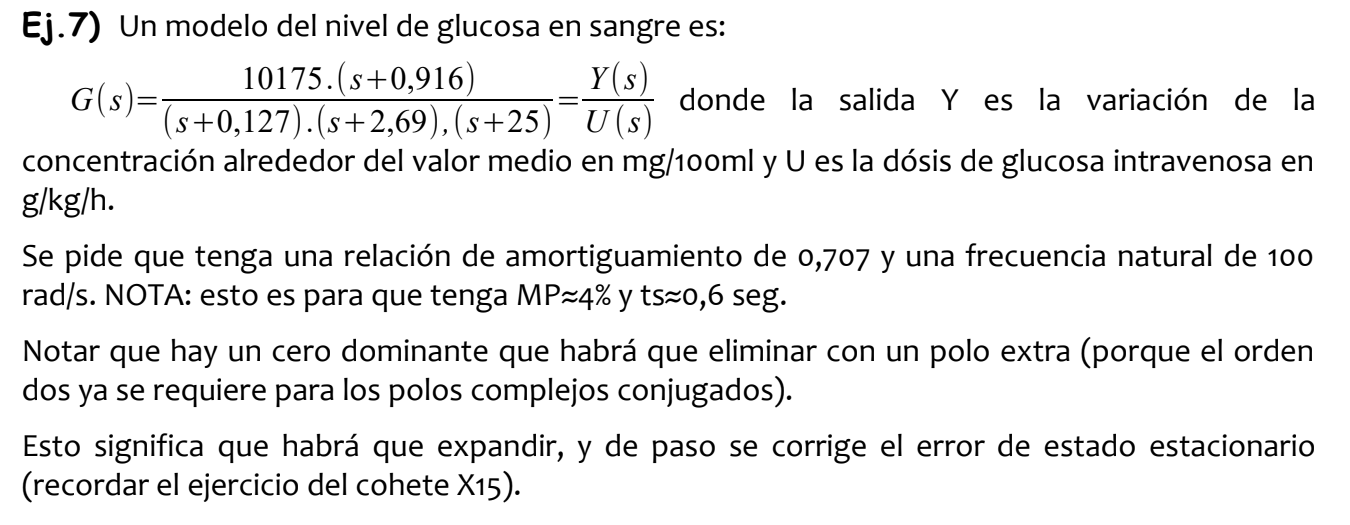
\includegraphics[width=\textwidth]{Imagenes/Ej7.png} \caption{Enunciado del Ejercicio 7.} \label{fig:enunciado_ej7} \end{figure}
Se busca controlar el nivel de glucosa en sangre mediante realimentación de estados, de modo que el sistema a lazo cerrado tenga una relación de amortiguamiento $\xi=0{,}707$ y una frecuencia natural $\omega_n=100\ \mathrm{rad/s}$.

La planta es:

\begin{equation}G(s)=\frac{Y(s)}{U(s)}=\frac{10175(s+0{,}916)}{(s+0{,}127)(s+2{,}69)(s+25)}\end{equation}
% ===== ESPECIFICACIONES =====
\subsection*{Especificaciones y polos deseados}
A partir de los parámetros pedidos:

\begin{equation}\sigma=\xi\omega_n=0{,}707\cdot100=70{,}7\end{equation}

\begin{equation}\omega_d=\omega_n\sqrt{1-\xi^2}=100\sqrt{1-0{,}707^2}\approx70{,}72\end{equation}

Por lo tanto, los polos dominantes deseados son:

\begin{equation}\boxed{p_{1,2}=-\sigma\pm j\omega_d=-70{,}7\pm j70{,}72}\end{equation}

El sobrepico y el tiempo de establecimiento del sistema de segundo orden correspondiente son:

\begin{equation}M_P=e^{-\xi\pi/\sqrt{1-\xi^2}}\approx4{,}3\,\text{\%}\end{equation}

\begin{equation}t_s\approx\frac{4}{\sigma}=\frac{4}{70{,}7}\approx0{,}057\ \mathrm{s}\end{equation}

El enunciado indica $t_s\approx0{,}6$ s, pero con $\sigma=70{,}7$ se obtiene $t_s\approx0{,}06$ s, por lo que se interpreta como un error de tipeo.

El polinomio de segundo orden asociado es:

\begin{equation}s^2+2\xi\omega_ns+\omega_n^2=s^2+141{,}4s+10000\end{equation}
% ===== ANALISIS DE LA PLANTA =====
\subsection*{Análisis de la planta}
\begin{itemize}
\item Polos: $-0{,}127$, $-2{,}69$ y $-25$. Todos se encuentran en el semiplano izquierdo, por lo que la planta es estable.
\item Cero: $-0{,}916$. Se encuentra muy cerca del origen en comparación con los polos deseados ($-70{,}7$), por lo que es un \textbf{cero dominante}. La realimentación de estados no modifica los ceros, de modo que este cero seguirá presente a lazo cerrado y deformará la respuesta si no se lo neutraliza.
\item La planta es de \textbf{tipo cero}, ya que no posee polos en el origen.
\end{itemize}

Su ganancia estática es:

\begin{equation}G(0)=\frac{10175\cdot0{,}916}{0{,}127\cdot2{,}69\cdot25}\approx1091\end{equation}
% ===== MODELO DE ESTADO =====
\subsection*{Modelo de estado}
\subsubsection*{Separación en bloques}
Cada polo se ubica en un bloque independiente, dejando el cero y la ganancia a la salida. Las variables de estado son las salidas de cada bloque, numeradas desde la salida:

\begin{equation}U\rightarrow\boxed{\frac{1}{s+25}}\xrightarrow{X_3}\boxed{\frac{1}{s+2{,}69}}\xrightarrow{X_2}\boxed{\frac{1}{s+0{,}127}}\xrightarrow{X_1}\boxed{10175(s+0{,}916)}\rightarrow Y\end{equation}
\subsubsection*{Obtención de las ecuaciones de estado}
\paragraph{Primera etapa: bloque $\boldsymbol{1/(s+25)}$.} Del diagrama:

\begin{equation}X_3(s)=U(s)\frac{1}{s+25}\end{equation}

Reordenando:

\begin{equation}sX_3(s)+25X_3(s)=U(s)\end{equation}

Aplicando transformada inversa de Laplace, con condiciones iniciales nulas:

\begin{equation}\boxed{\dot{x}_3=-25x_3+u}\end{equation}
\paragraph{Segunda etapa: bloque $\boldsymbol{1/(s+2{,}69)}$.} Del diagrama:

\begin{equation}X_2(s)=X_3(s)\frac{1}{s+2{,}69}\end{equation}

Reordenando:

\begin{equation}sX_2(s)+2{,}69X_2(s)=X_3(s)\end{equation}

Aplicando transformada inversa de Laplace:

\begin{equation}\boxed{\dot{x}_2=-2{,}69x_2+x_3}\end{equation}
\paragraph{Tercera etapa: bloque $\boldsymbol{1/(s+0{,}127)}$.} Del diagrama:

\begin{equation}X_1(s)=X_2(s)\frac{1}{s+0{,}127}\end{equation}

Reordenando:

\begin{equation}sX_1(s)+0{,}127X_1(s)=X_2(s)\end{equation}

Aplicando transformada inversa de Laplace:

\begin{equation}\boxed{\dot{x}_1=-0{,}127x_1+x_2}\end{equation}
\paragraph{Ecuación de salida.} El último bloque contiene el cero y la ganancia:

\begin{equation}Y(s)=10175(s+0{,}916)X_1(s)\end{equation}

En el dominio temporal:

\begin{equation}y=10175\dot{x}_1+9320{,}3x_1\end{equation}

En la ecuación de salida no puede aparecer una derivada, por lo que se reemplaza $\dot{x}_1=x_2-0{,}127x_1$:

\begin{equation}y=10175(x_2-0{,}127x_1)+9320{,}3x_1\end{equation}

Por lo tanto:

\begin{equation}\boxed{y=8028{,}1x_1+10175x_2}\end{equation}

El numerador de la planta queda contenido únicamente en la ecuación de salida.
\subsubsection*{Representación matricial}
Escribiendo las ecuaciones en forma matricial:

\begin{equation}\begin{bmatrix}\dot{x}_1\\\dot{x}_2\\\dot{x}_3\end{bmatrix}=\begin{bmatrix}-0{,}127&1&0\\0&-2{,}69&1\\0&0&-25\end{bmatrix} \begin{bmatrix}x_1\\x_2\\x_3\end{bmatrix}+\begin{bmatrix}0\\0\\1\end{bmatrix}u\end{equation}

\begin{equation}y=\begin{bmatrix}8028{,}1&10175&0\end{bmatrix} \begin{bmatrix}x_1\\x_2\\x_3\end{bmatrix}+0u\end{equation}

Por lo tanto:

\begin{equation}\boxed{A=\begin{bmatrix}-0{,}127&1&0\\0&-2{,}69&1\\0&0&-25\end{bmatrix} \qquad B=\begin{bmatrix}0\\0\\1\end{bmatrix}}\end{equation}

\begin{equation}\boxed{C=\begin{bmatrix}8028{,}1&10175&0\end{bmatrix} \qquad D=0}\end{equation}
\paragraph{Verificación.} Calculando $G(s)=C(sI-A)^{-1}B+D$ se obtiene:

\begin{equation}G(s)=\frac{10175s+9320{,}3}{s^3+27{,}817s^2+70{,}767s+8{,}541}=\frac{10175(s+0{,}916)}{(s+0{,}127)(s+2{,}69)(s+25)}\end{equation}

que coincide con la función de transferencia original.
% ===== NECESIDAD DE LA EXPANSION =====
\subsection*{Limitación de la realimentación de estados simple}
Con la ley de control vista en clase:

\begin{equation}u=r-K_1x_1-K_2x_2-K_3x_3=r-Kx\end{equation}

se pueden ubicar los tres polos de la planta. Si se eligen en $-70{,}7\pm j70{,}72$ y $-0{,}916$ (este último para cancelar el cero), el lazo cerrado resulta:

\begin{equation}T(s)=\frac{10175(s+0{,}916)}{(s^2+141{,}4s+10000)(s+0{,}916)}\end{equation}

Su valor en régimen permanente es:

\begin{equation}T(0)=\frac{9320{,}3}{0{,}916\cdot10000}=1{,}0175\end{equation}

Ante un escalón unitario la salida se establece en $1{,}0175$: el error de estado estacionario no es nulo. Esto se debe a que, con $u=r-Kx$, la referencia ingresa sin compararse con la salida, y nada garantiza que $y$ alcance a $r$.

Lo mismo ocurre en el ejercicio del cohete X15 visto en clase: allí se cancela el cero en $-0{,}4$ ubicando un polo de lazo cerrado sobre él, y la respuesta adopta la forma de segundo orden buscada, pero se establece en $T(0)=2/9\approx0{,}222$.

Para que la salida siga a la referencia se incorpora un integrador del error, es decir, se \textbf{expande} el sistema.
% ===== EXPANSION =====
\subsection*{Expansión del sistema}
Se agrega una cuarta variable de estado, que acumula el error entre la referencia y la salida:

\begin{equation}\dot{x}_4=r-y\end{equation}

Reemplazando la ecuación de salida:

\begin{equation}\boxed{\dot{x}_4=r-8028{,}1x_1-10175x_2}\end{equation}

La ley de control pasa a ser:

\begin{equation}\boxed{u=K_4x_4-K_1x_1-K_2x_2-K_3x_3}\end{equation}

El término $-K_1x_1-K_2x_2-K_3x_3$ es la realimentación de estados, que permite ubicar los polos. El término $K_4x_4$ corrige según el error acumulado: en régimen permanente $\dot{x}_4=0$, por lo que $r-y=0$ y la salida alcanza exactamente a la referencia.

La referencia $r$ ya no ingresa directamente en $u$, sino a través del integrador.
\subsubsection*{Ecuaciones de lazo cerrado}
Se reemplaza $u$ en la ecuación de $x_3$:

\begin{equation}\dot{x}_3=-25x_3+K_4x_4-K_1x_1-K_2x_2-K_3x_3\end{equation}

Agrupando:

\begin{equation}\dot{x}_3=-K_1x_1-K_2x_2-(25+K_3)x_3+K_4x_4\end{equation}

El sistema completo queda:

\begin{equation}\boxed{\begin{cases}\dot{x}_1=-0{,}127x_1+x_2\\\dot{x}_2=-2{,}69x_2+x_3\\\dot{x}_3=-K_1x_1-K_2x_2-(25+K_3)x_3+K_4x_4\\\dot{x}_4=-8028{,}1x_1-10175x_2+r\end{cases}}\end{equation}
\subsubsection*{Matriz de lazo cerrado}
Escribiendo las ecuaciones en forma matricial:

\begin{equation}\boxed{A_{LC}=\begin{bmatrix}-0{,}127&1&0&0\\0&-2{,}69&1&0\\-K_1&-K_2&-(25+K_3)&K_4\\-8028{,}1&-10175&0&0\end{bmatrix}}\end{equation}

\begin{equation}\dot{x}=A_{LC}x+\begin{bmatrix}0\\0\\0\\1\end{bmatrix}r \qquad y=\begin{bmatrix}8028{,}1&10175&0&0\end{bmatrix}x\end{equation}

En forma de bloques:

\begin{equation}A_{LC}=\begin{bmatrix}A-BK&BK_4\\-C&0\end{bmatrix}\end{equation}

La fila agregada es $-C$: el numerador de la planta ingresa a la matriz a través del integrador.
% ===== CONTROLABILIDAD =====
\subsection*{Controlabilidad}
Antes de ubicar los polos se verifica que el sistema expandido sea controlable mediante el test de Kalman:

\begin{equation}A_e=\begin{bmatrix}A&0\\-C&0\end{bmatrix} \qquad B_e=\begin{bmatrix}B\\0\end{bmatrix}\end{equation}

\begin{equation}M_C=\begin{bmatrix}B_e&A_eB_e&A_e^2B_e&A_e^3B_e\end{bmatrix}\end{equation}

Calculando:

\begin{equation}M_C=\begin{bmatrix}0&0&1&-27{,}817\\0&1&-27{,}69&699{,}49\\1&-25&625&-15625\\0&0&-10175&273717{,}7\end{bmatrix}\end{equation}

\begin{equation}\boxed{|M_C|=9320{,}3\neq0}\end{equation}

Por lo tanto, el sistema expandido es completamente controlable y pueden ubicarse sus cuatro polos.
% ===== ECUACION CARACTERISTICA =====
\subsection*{Ecuación característica}
Se calcula $|sI-A_{LC}|$:

\begin{equation}sI-A_{LC}=\begin{bmatrix}s+0{,}127&-1&0&0\\0&s+2{,}69&-1&0\\K_1&K_2&s+25+K_3&-K_4\\8028{,}1&10175&0&s\end{bmatrix}\end{equation}

Se desarrolla por la cuarta columna, que posee dos ceros. Los signos de los cofactores siguen el patrón:

\begin{equation}\begin{bmatrix}+&-&+&-\\-&+&-&+\\+&-&+&-\\-&+&-&+\end{bmatrix}\end{equation}
\paragraph{Término del elemento $\boldsymbol{(4,4)=s}$, signo $+$.} Se elimina la fila 4 y la columna 4:

\begin{equation}s\cdot\begin{vmatrix}s+0{,}127&-1&0\\0&s+2{,}69&-1\\K_1&K_2&s+25+K_3\end{vmatrix}\end{equation}

Desarrollando por la primera columna:

\begin{equation}(s+0{,}127)\left[(s+2{,}69)(s+25+K_3)+K_2\right]+K_1\end{equation}

Como $(s+0{,}127)(s+2{,}69)=s^2+2{,}817s+0{,}3416$:

\begin{equation}s^3+(27{,}817+K_3)s^2+(70{,}767+2{,}817K_3+K_2)s+(8{,}541+0{,}3416K_3+0{,}127K_2+K_1)\end{equation}
\paragraph{Término del elemento $\boldsymbol{(3,4)=-K_4}$, signo $-$.} Se elimina la fila 3 y la columna 4:

\begin{equation}-(-K_4)\cdot\begin{vmatrix}s+0{,}127&-1&0\\0&s+2{,}69&-1\\8028{,}1&10175&0\end{vmatrix}\end{equation}

Desarrollando por la tercera columna, solo aporta el elemento $(2,3)=-1$, con signo $-$:

\begin{equation}-(-1)\begin{vmatrix}s+0{,}127&-1\\8028{,}1&10175\end{vmatrix}=10175(s+0{,}127)+8028{,}1=10175s+9320{,}3\end{equation}

que es el numerador de la planta. Este término vale $K_4(10175s+9320{,}3)$.
\paragraph{Resultado.} Sumando ambos términos:

\begin{equation}\boxed{\begin{aligned}|sI-A_{LC}|={}&s^4+(27{,}817+K_3)s^3+(70{,}767+2{,}817K_3+K_2)s^2\\&+(8{,}541+0{,}3416K_3+0{,}127K_2+K_1+10175K_4)s+9320{,}3K_4\end{aligned}}\end{equation}
% ===== ELECCION DE POLOS =====
\subsection*{Elección de los polos de lazo cerrado}
Como $A_{LC}$ es de $4\times4$, deben ubicarse cuatro polos:

\begin{itemize}
\item $-70{,}7\pm j70{,}72$: cumplen $\xi=0{,}707$ y $\omega_n=100$, según lo pedido por el enunciado.
\item $-0{,}916$: coincide con el cero de la planta y lo cancela en la transferencia de lazo cerrado. Es el ``polo extra'' que menciona el enunciado.
\item $-700$: polo sobrante de la expansión. Se ubica aproximadamente diez veces más lejos del eje imaginario que la parte real de los polos dominantes ($10\cdot70{,}7\approx700$), para que su modo se extinga rápidamente y no afecte la respuesta.
\end{itemize}

No es posible igualar utilizando solo tres polos, ya que la ecuación característica es de grado cuatro y existen cuatro incógnitas. Tampoco conviene utilizar un polo de la planta como $-25$, ya que se encuentra más cerca del eje imaginario que $-70{,}7$ y pasaría a dominar la respuesta.

El polinomio deseado es:

\begin{equation}P_d(s)=(s^2+141{,}4s+10000)(s+0{,}916)(s+700)\end{equation}

Multiplicando primero los factores reales:

\begin{equation}(s+0{,}916)(s+700)=s^2+700{,}916s+641{,}2\end{equation}

Por lo tanto:

\begin{equation}P_d(s)=(s^2+141{,}4s+10000)(s^2+700{,}916s+641{,}2)\end{equation}

\begin{equation}\boxed{P_d(s)=s^4+842{,}316s^3+109750{,}7s^2+7099825{,}7s+6412000}\end{equation}
% ===== CALCULO DE GANANCIAS =====
\subsection*{Cálculo de las ganancias}
Se igualan los coeficientes de $|sI-A_{LC}|$ y $P_d(s)$, comenzando por el término independiente, que contiene una única incógnita.
\paragraph{Término $\boldsymbol{s^0}$.}

\begin{equation}9320{,}3K_4=6412000\Rightarrow\boxed{K_4=687{,}96}\end{equation}
\paragraph{Término $\boldsymbol{s^3}$.}

\begin{equation}27{,}817+K_3=842{,}316\Rightarrow\boxed{K_3=814{,}50}\end{equation}
\paragraph{Término $\boldsymbol{s^2}$.}

\begin{equation}70{,}767+2{,}817\cdot814{,}50+K_2=109750{,}7\end{equation}

\begin{equation}70{,}767+2294{,}4+K_2=109750{,}7\Rightarrow\boxed{K_2=107385{,}5}\end{equation}
\paragraph{Término $\boldsymbol{s^1}$.} Se utiliza que $10175K_4=6412000/0{,}916=7000000$, ya que $9320{,}3=10175\cdot0{,}916$:

\begin{equation}8{,}541+0{,}3416\cdot814{,}50+0{,}127\cdot107385{,}5+K_1+7000000=7099825{,}7\end{equation}

\begin{equation}8{,}541+278{,}3+13638{,}0+K_1+7000000=7099825{,}7\Rightarrow\boxed{K_1=85900{,}9}\end{equation}

Por lo tanto, la ley de control resulta:

\begin{equation}\boxed{u=687{,}96x_4-85900{,}9x_1-107385{,}5x_2-814{,}50x_3}\end{equation}
% ===== VERIFICACIONES =====
\subsection*{Verificaciones}
\subsubsection*{Autovalores de la matriz de lazo cerrado}
Reemplazando las ganancias:

\begin{equation}A_{LC}=\begin{bmatrix}-0{,}127&1&0&0\\0&-2{,}69&1&0\\-85900{,}9&-107385{,}5&-839{,}50&687{,}96\\-8028{,}1&-10175&0&0\end{bmatrix}\end{equation}

Sus autovalores son:

\begin{equation}\boxed{\lambda_{1,2}=-70{,}7\pm j70{,}72,\qquad \lambda_3=-0{,}916,\qquad \lambda_4=-700}\end{equation}

que coinciden con los polos elegidos.
\subsubsection*{Transferencia de lazo cerrado}
\begin{equation}T(s)=\frac{K_4(10175s+9320{,}3)}{|sI-A_{LC}|}=\frac{7000000(s+0{,}916)}{(s^2+141{,}4s+10000)(s+0{,}916)(s+700)}\end{equation}

El factor $(s+0{,}916)$ se cancela, por lo que el cero dominante deja de afectar la respuesta:

\begin{equation}\boxed{T(s)=\frac{7000000}{(s^2+141{,}4s+10000)(s+700)}}\end{equation}

Como el polo en $-700$ está alejado, el sistema se comporta como el segundo orden buscado. Además:

\begin{equation}T(0)=\frac{7000000}{10000\cdot700}=1\end{equation}

por lo que el error de estado estacionario al escalón es nulo.
\subsubsection*{Estabilidad por Routh-Hurwitz}
Para el polinomio característico obtenido:

\begin{equation}\begin{array}{c|ccc}s^4&1&109750{,}7&6412000\\s^3&842{,}316&7099825{,}7&0\\s^2&101321{,}8&6412000&\\s^1&7046521{,}0&&\\s^0&6412000&&\end{array}\end{equation}

No hay cambios de signo en la primera columna, por lo que el sistema a lazo cerrado es estable, como era de esperar al haber ubicado todos los polos en el semiplano izquierdo.
\subsubsection*{Respuesta al escalón}
Descomponiendo $T(s)/s$ en fracciones parciales y antitransformando, la respuesta al escalón unitario es:

\begin{equation}\boxed{y(t)=1-0{,}0249e^{-700t}-e^{-70{,}7t}\left[0{,}9751\cos(70{,}72t)+1{,}2216\sin(70{,}72t)\right]}\end{equation}

Para comparar, el segundo orden ideal y el diseño sin integrador ($u=r-Kx$) responden según:

\begin{equation}y_{\mathrm{ideal}}(t)=1-e^{-70{,}7t}\left[\cos(70{,}72t)+0{,}9997\sin(70{,}72t)\right]\end{equation}

\begin{equation}y_{\mathrm{sin\ int}}(t)=1{,}0175\,y_{\mathrm{ideal}}(t)\end{equation}

\begin{figure}[H]\centering\begin{tikzpicture}\begin{axis}[width=0.9\textwidth, height=7cm, xlabel={Tiempo (ms)}, ylabel={Salida $y(t)$}, title={Respuesta al escalón unitario}, xmin=0, xmax=150, ymin=0, ymax=1.12, grid=both, major grid style={gray!35}, minor grid style={gray!15}, legend pos=south east, line width=1pt, trig format plots=rad]
\addplot[blue, thick, domain=0:150, samples=300]{1-0.02494*exp(-0.7*x)-exp(-0.0707*x)*(0.97506*cos(0.07072*x)+1.22159*sin(0.07072*x))};\addlegendentry{Diseño con integrador}
\addplot[black, dashed, domain=0:150, samples=300]{1-exp(-0.0707*x)*(cos(0.07072*x)+0.9997*sin(0.07072*x))};\addlegendentry{Segundo orden ideal}
\addplot[red, dotted, thick, domain=0:150, samples=300]{1.0175*(1-exp(-0.0707*x)*(cos(0.07072*x)+0.9997*sin(0.07072*x)))};\addlegendentry{Sin integrador ($u=r-Kx$)}
\end{axis}\end{tikzpicture}\caption{Respuesta al escalón unitario del diseño, del segundo orden ideal y del diseño sin integrador.}\end{figure}

Los valores obtenidos son:

\begin{table}[H]\centering\begin{tabular}{lccc}\hline & Diseño & Segundo orden ideal & Sin integrador\\\hline Sobrepico $M_P$ & $4{,}28\,\text{\%}$ & $4{,}33\,\text{\%}$ & --- \\ Tiempo de pico $t_p$ & $46$ ms & $44$ ms & --- \\ Tiempo de establecimiento $t_s$ ($2\,\text{\%}$) & $61$ ms & $60$ ms & --- \\ Valor final & $1$ & $1$ & $1{,}0175$\\ Error de estado estacionario & $0$ & $0$ & $-1{,}75\,\text{\%}$\\\hline\end{tabular}\caption{Parámetros de la respuesta al escalón.}\end{table}

El diseño reproduce prácticamente la respuesta del segundo orden ideal, y el integrador elimina el error que presenta la versión sin expansión.
\subsubsection*{Influencia del cuarto polo}
Si el cuarto polo se ubica en $-350$ (cinco veces la parte real dominante), las ganancias resultan:

\begin{equation}K_1=46888{,}4 \qquad K_2=58560{,}9 \qquad K_3=464{,}50 \qquad K_4=343{,}98\end{equation}

y la respuesta al escalón es:

\begin{equation}y(t)=1-0{,}1205e^{-350t}-e^{-70{,}7t}\left[0{,}8795\cos(70{,}72t)+1{,}4755\sin(70{,}72t)\right]\end{equation}

\begin{figure}[H]\centering\begin{tikzpicture}\begin{axis}[width=0.9\textwidth, height=7cm, xlabel={Tiempo (ms)}, ylabel={Salida $y(t)$}, title={Comparación según la ubicación del cuarto polo}, xmin=0, xmax=150, ymin=0, ymax=1.12, grid=both, major grid style={gray!35}, minor grid style={gray!15}, legend pos=south east, line width=1pt, trig format plots=rad]
\addplot[blue, thick, domain=0:150, samples=300]{1-0.02494*exp(-0.7*x)-exp(-0.0707*x)*(0.97506*cos(0.07072*x)+1.22159*sin(0.07072*x))};\addlegendentry{$p_4=-700$}
\addplot[orange, thick, dashed, domain=0:150, samples=300]{1-0.12047*exp(-0.35*x)-exp(-0.0707*x)*(0.87953*cos(0.07072*x)+1.47546*sin(0.07072*x))};\addlegendentry{$p_4=-350$}
\end{axis}\end{tikzpicture}\caption{Respuesta al escalón para dos ubicaciones del cuarto polo.}\end{figure}

Con $p_4=-350$ las ganancias se reducen aproximadamente a la mitad, con un sobrepico de $4{,}10\,\text{\%}$ y $t_s\approx63$ ms. La respuesta prácticamente no cambia, por lo que la elección del cuarto polo es un compromiso entre su influencia en la respuesta y el esfuerzo de control.
\subsubsection*{Señal de control}
La transferencia entre la referencia y la entrada a la planta es:

\begin{equation}\frac{U(s)}{R(s)}=\frac{T(s)}{G(s)}=\frac{K_4(s+0{,}127)(s+2{,}69)(s+25)}{P_d(s)}\end{equation}

Antitransformando la respuesta al escalón:

\begin{equation}\begin{aligned}u(t)={}&0{,}000916+0{,}00367e^{-0{,}916t}-1{,}1548e^{-700t}\\&+e^{-70{,}7t}\left[1{,}1503\cos(70{,}72t)-0{,}5528\sin(70{,}72t)\right]\end{aligned}\end{equation}

\begin{figure}[H]\centering\begin{tikzpicture}\begin{axis}[width=0.9\textwidth, height=6.5cm, xlabel={Tiempo (ms)}, ylabel={Entrada $u(t)$}, title={Señal de control ante un escalón en la referencia}, xmin=0, xmax=150, grid=both, major grid style={gray!35}, minor grid style={gray!15}, legend pos=north east, line width=1pt, trig format plots=rad]
\addplot[blue, thick, domain=0:150, samples=400]{0.000916+0.003669*exp(-0.000916*x)-1.15483*exp(-0.7*x)+exp(-0.0707*x)*(1.15025*cos(0.07072*x)-0.55282*sin(0.07072*x))};\addlegendentry{$p_4=-700$}
\end{axis}\end{tikzpicture}\caption{Dosis de glucosa aplicada a la planta ante un escalón unitario en la referencia.}\end{figure}

La cancelación del polo en $-0{,}916$ ocurre en la transferencia $r\rightarrow y$, pero no en $r\rightarrow u$. Por ese motivo $u(t)$ presenta una componente lenta, con constante de tiempo $\tau\approx1/0{,}916\approx1{,}1$ s, que tiende a $u_{ss}=1/G(0)\approx9{,}2\cdot10^{-4}$. La salida no la percibe, pero constituye un modo interno del sistema.
% ===== CONCLUSIONES =====
\subsection*{Conclusiones}
La realimentación de estados permite ubicar los polos del sistema en cualquier posición, pero no modifica los ceros de la planta. El cero dominante en $-0{,}916$ se neutralizó ubicando un polo de lazo cerrado sobre él.

Como ocurre en el ejercicio del cohete X15, la ley de control $u=r-Kx$ deja un error de estado estacionario ($y_{ss}=1{,}0175$). La expansión del sistema mediante un integrador del error ($\dot{x}_4=r-y$) lo elimina.

El sistema expandido resulta de orden cuatro: dos polos para el par complejo dominante, uno para cancelar el cero y uno libre, ubicado lejos del eje imaginario. Las ganancias obtenidas son:

\begin{equation}\boxed{K_1=85900{,}9 \qquad K_2=107385{,}5 \qquad K_3=814{,}50 \qquad K_4=687{,}96}\end{equation}

Las simulaciones confirman un sobrepico de $4{,}3\,\text{\%}$, un tiempo de establecimiento de $0{,}06$ s y error de estado estacionario nulo, y el criterio de Routh-Hurwitz confirma la estabilidad del sistema a lazo cerrado.

\end{document}
